\documentclass[5p]{elsarticle}
\usepackage{xspace}
\usepackage{lineno,hyperref}
\usepackage{url}
\usepackage{CJKutf8}
\usepackage{xcolor}
\usepackage[xcolor=dvipdf]{changes}
% \usepackage[xcolor=dvipdf, final]{changes}
\definecolor{mygreen}{rgb}{0.17, 0.55, 0.05}
\definechangesauthor[name=JiachengPan, color=mygreen]{pan}
\setdeletedmarkup{\color{gray}{#1}}
\modulolinenumbers[5]

\journal{Journal of \LaTeX\ Templates}

%%%%%%%%%%%%%%%%%%%%%%%
%% Elsevier bibliography styles
%%%%%%%%%%%%%%%%%%%%%%%
%% To change the style, put a % in front of the second line of the current style and
%% remove the % from the second line of the style you would like to use.
%%%%%%%%%%%%%%%%%%%%%%%

%% Numbered
%\bibliographystyle{model1-num-names}

%% Numbered without titles
%\bibliographystyle{model1a-num-names}

%% Harvard
%\bibliographystyle{model2-names.bst}\biboptions{authoryear}

%% Vancouver numbered
%\usepackage{numcompress}\bibliographystyle{model3-num-names}

%% Vancouver name/year
%\usepackage{numcompress}\bibliographystyle{model4-names}\biboptions{authoryear}

%% APA style
%\bibliographystyle{model5-names}\biboptions{authoryear}

%% AMA style
%\usepackage{numcompress}\bibliographystyle{model6-num-names}

%% `Elsevier LaTeX' style
\bibliographystyle{elsarticle-num}
%%%%%%%%%%%%%%%%%%%%%%%
\newcommand{\name}{NetV.js\xspace}

\begin{document}
\begin{CJK}{UTF8}{gbsn}
\begin{frontmatter}

\title{\name: A Large-Scale Graph Visualization Library}
% \tnotetext[mytitlenote]{Fully documented templates are available in the elsarticle package on \href{http://www.ctan.org/tex-archive/macros/latex/contrib/elsarticle}{CTAN}.}

%% Group authors per affiliation:
% \author{Elsevier1,2}
% \address{Radarweg 29, Amsterdam}
% \author{Elsevier3}
% \address{Radarweg 29, Amsterdam}
%% or include affiliations in footnotes:
\author[mymainaddress,mysecondaryaddress]{Dongming Han, Jiacheng Pan, Rusheng Pan, Jiehui Zhou, Xiaodong Zhao}
\author[mymainaddress]{Wei Chen\corref{mycorrespondingauthor}}
\cortext[mycorrespondingauthor]{Corresponding author}
\ead{chenvis@zju.edu.cn}

\address[mymainaddress]{State Key Lab of CAD\&CG, Zhejiang University, Hangzhou, Zhejiang, China}
\address[mysecondaryaddress]{Zhejiang Lab, hangzhou, zhejiang, China}

\begin{abstract}
    Network visualization plays an important role in many fields, such as social media networks, protein-protein-interaction networks, and traffic networks. In the meantime, a dozen of visualization designer tools and programming toolkits are widely used in implementing network visualization applications. With network data growth, exiting tools can not help users rapidly and efficiently construct large-scale network visualization.
    In this paper, we present \name, an open-sourced, JavaScript-based, WebGL-based library that supports the rapid large-scale network rendering, interaction, and visualization.
    
\end{abstract}

\begin{keyword}
Network visualization\sep Web-based visualization
\end{keyword}

\end{frontmatter}

\linenumbers

\section{Introduction}
\deleted[id=pan]{图数据在现实世界广泛存在。图数据的可视化在很多领域都有其重要作用,比如在金融数据可视分析中可视化欺诈交易,探索社交媒体网络中的信息传播,以及展示生物网络中的蛋白质互相作用等等。
为了提升用户和开发者构建可视化的效率,一系列可视化构建工具被提出。特别是d3的提出,降低了基于web的可视化构建的难度,丰富了可视化社区。因此,很多图数据可视化工具也基于web进行开发。其中,节点链接图是最为广泛使用的可视化形式。}

\added[id=pan]{Graph visualization plays an important role in many fields, such as showing fraud transactions in financial data analysis~\cite{DBLP:journals/tvcg/ChenGHPNXZ19}, exploring information propagation in social media graph~\cite{DBLP:conf/candt/SmithSMRBDCPG09}, and visualizing protein-protein-interaction in biological graph~\cite{doncheva2012topological}.
A series of visualization authoring tools~\cite{satyanarayan2014declarative,mendez2016ivolver,kim2016data} have been developed to facilitate visualization generation~\cite{lu2020illustrating,lyra,lyra2}. Notably, the proposal of d3.js~\cite{DBLP:journals/tvcg/BostockOH11} reduces the difficulty of web-based visualization authoring and enriches the visualization community. Thus, many graph visualization tools are also web-based. Node-link diagrams are widely used among many graph visualization solutions~\cite{pan2020rcanalyzer}, because they reveal topology and connectivities~\cite{ghoniem2004comparison}.}
% graph data wildly exists in the world. graph visualization plays an important role in many fields, such as showing fraud transactions in financial data analysis~\cite{DBLP:journals/tvcg/ChenGHPNXZ19}, exploring information propagation in social media graph~\cite{DBLP:conf/candt/SmithSMRBDCPG09}, and visualizing protein-protein-interaction in biological graph~\cite{doncheva2012topological}. As the development of modern browsers and open-sourced communities, a series of visualization generation tools and programming toolkits are employed to construct graph visualization in a web page~\cite{DBLP:journals/tvcg/SrinivasanPEB18,DBLP:conf/ieeevast/BigelowNML19}. In the meantime, as the data grows, attention has been paid to the large-scale graph visualization~\cite{DBLP:journals/tvcg/ChenGHPNXZ19}. A series of requirements and tasks requires developers to explore and analyze large graphs. A large-scale graph visualization tool is necessary for developers to rapidly and efficiently construct systems.
\deleted[id=pan]{节点链接图可视化拥有其特点,比如每一条链接往往链接了两个节点,用户只需控制节点的位置,其链接的位置会相应变化;节点链接图依赖于布局算法,从图数据到可视化的映射,需要用户通过布局算法来处理节点的位置摆放;针对节点的交互(比如点击和拖拽)非常普遍。开发者在使用通用的可视化工具进行开发时,需要pay effort to 处理这些问题。比如在使用D3.js进行图数据可视化时,开发者需要使用其数据驱动文档的思想将对应的数据映射到对应的可视化元素上,开发者直接面向可视化元素进行开发,没有抽象的模型来支持他控制整个图数据,可能会导致编程错误的产生。
一些图可视化构建工具,比如xxxx,良好地支持了对图数据的可视化,相对于通用的可视化工具而言,他们通过解决节点链接图的特殊需求,封装图可视化的相关接口,隐藏一部分开发者不关心的接口(比如对边的位置控制),暴露一部分图可视化特性接口(对相邻节点的访问),来提升自身的易用性。}
\added[id=pan]{developers only need to control the nodes' positions and related links change their positions correspondingly. Node-link diagrams strongly rely on layout algorithms. In the meantime, interactions on nodes such as clicking and dragging are frequently needed. Developers need to pay special attention on these aspects using general visualization authoring tools such as d3.js~\cite{DBLP:journals/tvcg/BostockOH11}, p4~\cite{p4,DBLP:journals/tvcg/LiM20,p6}, and stardust~\cite{DBLP:journals/cgf/RenLH17}.
For example, using d3.js to create a node-link diagram needs to map data elements to graphical marks by means of the data-drive-documents scheme. The developer needs to directly handle visual elements and there is no hook/handler to handle the underlying graph. It may lead to bugs.
Some graph visualization authoring tools such as Cytoscape.js~\cite{DBLP:journals/bioinformatics/FranzLHDSB16} and Sigma.js~\cite{DBLP:journals/jossw/Coene18} support graph visualization efficiently. Compared to general visualization tools, they encapsulate related interfaces of graph visualization, hide unrelated interfaces (e.g. controlling the position of a link) for developers, and expose some graph-related interfaces (e.g. accessing neighborhoods of a node). They improve the usability by leveraging the features of node-link diagrams.}

\deleted[id=pan]{随着数据规模的增长,图可视化也需要处理更多graphical marks(比如节点和链接)。然而,现有大部分图可视化工具难以处理有较多graphical marks。根据我们的实验,它们在渲染较大规模数据集上存在延迟,这将会降低用户的accessibility。}

\added[id=pan]{For large-scale graphs, a large amount of graphical marks (e.g., nodes and edges) need to be processed. However, most tools have a limited capability in displaying graph data in real-time. According to our experiments in Section~\ref{sec:experiment}, a heavy delay occurs in visualizing graphs which have more than 5 thousand elements, leading unpleasing user experiences.}

% One main bottleneck of visualizing large-scale graphs is the rendering performance. Conventional tools use DOM tree, SVG, or Canvas to construct graph visualization, such as D3.js~\cite{DBLP:journals/tvcg/BostockOH11}, Cytoscape.js~\cite{DBLP:journals/bioinformatics/FranzLHDSB16}, and Echarts~\cite{DBLP:journals/vi/LiMSSZWZC18}. They can not handle a large number of elements.

% For example, the SVG performance test of D3.js indicates that rendering 2000 elements will cause a noticeable lack of smoothness (around 24 frames per second)~\cite{svg}. For optimizing the effectiveness of rendering, D3.js supports Canvas in its fifth version. Echarts and Fabric.js also use Canvas as their rendering backend. However, the Canvas performance test shows that 10,000 elements will cause an obvious lack of smoothness~\cite{canvas}.
% Now, continuous research and tools focus on rendering data by using WebGL (GPU), such as Stardust.js~\cite{DBLP:journals/cgf/RenLH17}, PixiJS~\cite{graphicslearn} and P5~\cite{DBLP:journals/tvcg/LiM20}. WebGL takes a remarkable efficiency improvement in rendering, but the challenge of WebGL programming difficulty also comes.
% developers need to master the knowledge of graphics pipeline and shader programming.
% The steer learning curve and complex API lead to the second challenge.
% It is difficult for developers to construct graph visualizations easily.
% Existing WebGL-based visualization generation tools have already
% encapsulated a series of API about bottom interfaces. And they aim to generate general visualization components. As a result, they are inevitable to design complex and diverse API for adapting the requirements of different visualizations.
% Complex API will hinder developers who have no experience of visualization in constructing graph visualization applications. Sometimes, developers still need to write some shader related codes.
% In the meantime, the goal of generality needs a lot of logic code and complex data structure.
% The rendering and interaction performance will be greatly reduced in a specified visualization task due to the redundancy in design.
% It is still a difficult task for developers to construct large-scale graph visualization rapidly and efficiently.

\deleted[id=pan]{据我们所知,尚未存在一款工具,能够解决开发者易用性以及用户可访问性的问题。我们探索了图可视化的相关设计需求,设计并实现了NetV,一款基于web的高性能图可视化工具。其通过设计一系列图可视化相关的功能和接口来提高开发者易用性,并调用了GPU的高性能渲染能力来提高渲染效率以增加用户的可访问性。
通过和其他工具的对比实验,我们验证了NetV的accessibility和usability。
我们对该工具进行了开源以便开发者访问和贡献代码。}

\added[id=pan]{To the best of our knowledge, no existing tool can meet the requirements of developer usability and user accessibility at the same time. We analyze the design requirements of node-link diagram visualization, design and implement \name, a web-based high-performance node-link diagram visualization library. It provides the developer usability by means of a suite of node-link related features and interfaces and increases user accessibility by utilizing the high-performance rendering ability of GPU.
We evaluate the usability and accessibility of our implementation with comparative experiments.
We contribute \name, an open source library online (\url{https://netv.zjuvag.org/}).}

% To address performance and accessibility challenges, we designed and developed \name, an open-sourced\footnote{\url{netv.zjuvag.org}}, JavaScript-based, WebGL-based library for rapidly and easily construct large-scale graph visualization. \name leverages GPU processing power to render large-scale graph and provide rich build-in interactions to explore graphs. At the same time, \name own friendly and concise programming interfaces for developers to rapidly construct graph visualization applications.
\section{Related Work}
% \subsection{Web-based Visualization Authoring Tools}

% \subsection{Graph Visualization Authoring Tools}
Many libraries~\cite{DBLP:journals/vi/LiMSSZWZC18,mei2020datav,tableau} (tools, grammars, and frameworks) have been provided for implementing graph-based applications~\cite{wang2018graphprotector,pan2020exemplar}.
At the beginning, developers use conventional programming languages to construct graph visualization applications, such as C Sharp, C++, Javascript, and Python. Developers need to have proficient programming skills and understand the implementation mechanism~\cite{reas2003processing,reas2005processing}.
In the meantime, they also spend a lot of time developing and debugging. To make it easier for developers to program and develop quickly, visualization grammars and frameworks~\cite{lyra,lyra2,heer2010declarative} allows for detailed configurations on visual channels of visualizations such as D3.js~\cite{DBLP:journals/tvcg/BostockOH11}, ECharts~\cite{DBLP:journals/vi/LiMSSZWZC18}, Vega~\cite{DBLP:journals/tvcg/SatyanarayanRHH16}, and Vega-Lite~\cite{DBLP:journals/tvcg/SatyanarayanMWH17}.


However, when developers construct graph visualizations, they need to carefully select complex and different API to construct a graph, because these APIs are designed for full visualization rather than graph visualization applications. Cytoscape.js~\cite{DBLP:journals/bioinformatics/FranzLHDSB16}, Sigma.js~\cite{DBLP:journals/jossw/Coene18} and Gephi~\cite{DBLP:conf/icwsm/BastianHJ09} are used to construct graph visualizations. They encapsulate a series of API which are elaborated for the graph data. Developers can use them to construct graph visualizations quickly.
Moreover, large-scale data brings new challenges.
Some libraries~\cite{heer2005prefuse,wickham2011ggplot2,ren2014ivisdesigner} use Canvas to render elements.
However, these libraries can only render thousands of elements. To address this issue, PixiJS~\cite{graphicslearn}, P5~\cite{DBLP:journals/tvcg/LiM20} and Stardust~\cite{DBLP:journals/cgf/RenLH17} use GPU-based acceleration technology to render a large number of elements.
However, these GPU-based tools are also not designed for graph visualizations.
They still have redundancy and complex API that have nothing to do with graph visualizations. It leads to a decrease in rendering efficiency and an increase in learning costs.

\name targets on high-efficient visualization of large-scale node-link diagrams. It leverages a GPU-based visualization framework to improve the rendering performance, and design-friendly concise programming interfaces for efficient manipulation over graph elements.

% \subsection{graph Grammars and Frameworks}
% Many graph grammars and frameworks have been provided to developers for designing graph visualization applications.
% In the beginning, developers use conventional programming languages to construct graph visualization applications, such as C Sharp, C++, Javascript, and Python. Developers need to have proficient programming skills and understand the implementation mechanism.
% In the meantime, they also spend a lot of time developing and debugging. To make it easier for developers to program and develop quickly, visualization grammars and frameworks give granular control of visual channels of visualizations such as D3.js~\cite{DBLP:journals/tvcg/BostockOH11}, ECharts~\cite{DBLP:journals/vi/LiMSSZWZC18}, Vega~\cite{DBLP:journals/tvcg/SatyanarayanRHH16}, and Vega-Lite~\cite{DBLP:journals/tvcg/SatyanarayanMWH17}. Developers can use more concise tools to construct visualizations.


% However, when developers construct graph visualizations, they need to carefully select complex and different API to construct a graph, because these APIs are designed for full visualization rather than graph visualization applications. Cytoscape.js~\cite{DBLP:journals/bioinformatics/FranzLHDSB16}, sigmajs~\cite{DBLP:journals/jossw/Coene18} and Gephi~\cite{DBLP:conf/icwsm/BastianHJ09} are used to construct graph visualizations. They encapsulate a series of API which are elaborated for the graph data. Developers can use them to construct graph visualizations quickly.
% Moreover, large-scale data brings new challenges. These grammars and tools can only render thousands of elements. To address this issue, PixiJS~\cite{graphicslearn}, P5~\cite{DBLP:journals/tvcg/LiM20} and Stardust~\cite{DBLP:journals/cgf/RenLH17} used GPU-based acceleration technology to render a large number of elements.
% However, these GPU-based tools are also not designed for graph visualizations.
% They still have redundancy and complex API that have nothing to do with graph visualizations. It leads to a decrease in rendering efficiency and an increase in learning costs.

% Our \name focus on large-scale graph visualization. It uses a GPU-based rendering engine to support large-scale data and design-friendly concise programming interfaces for graph visualization construction.

% \subsection{GPU-based Visualization Rendering}





\section{\name Design}
\begin{figure*}[htbp]
    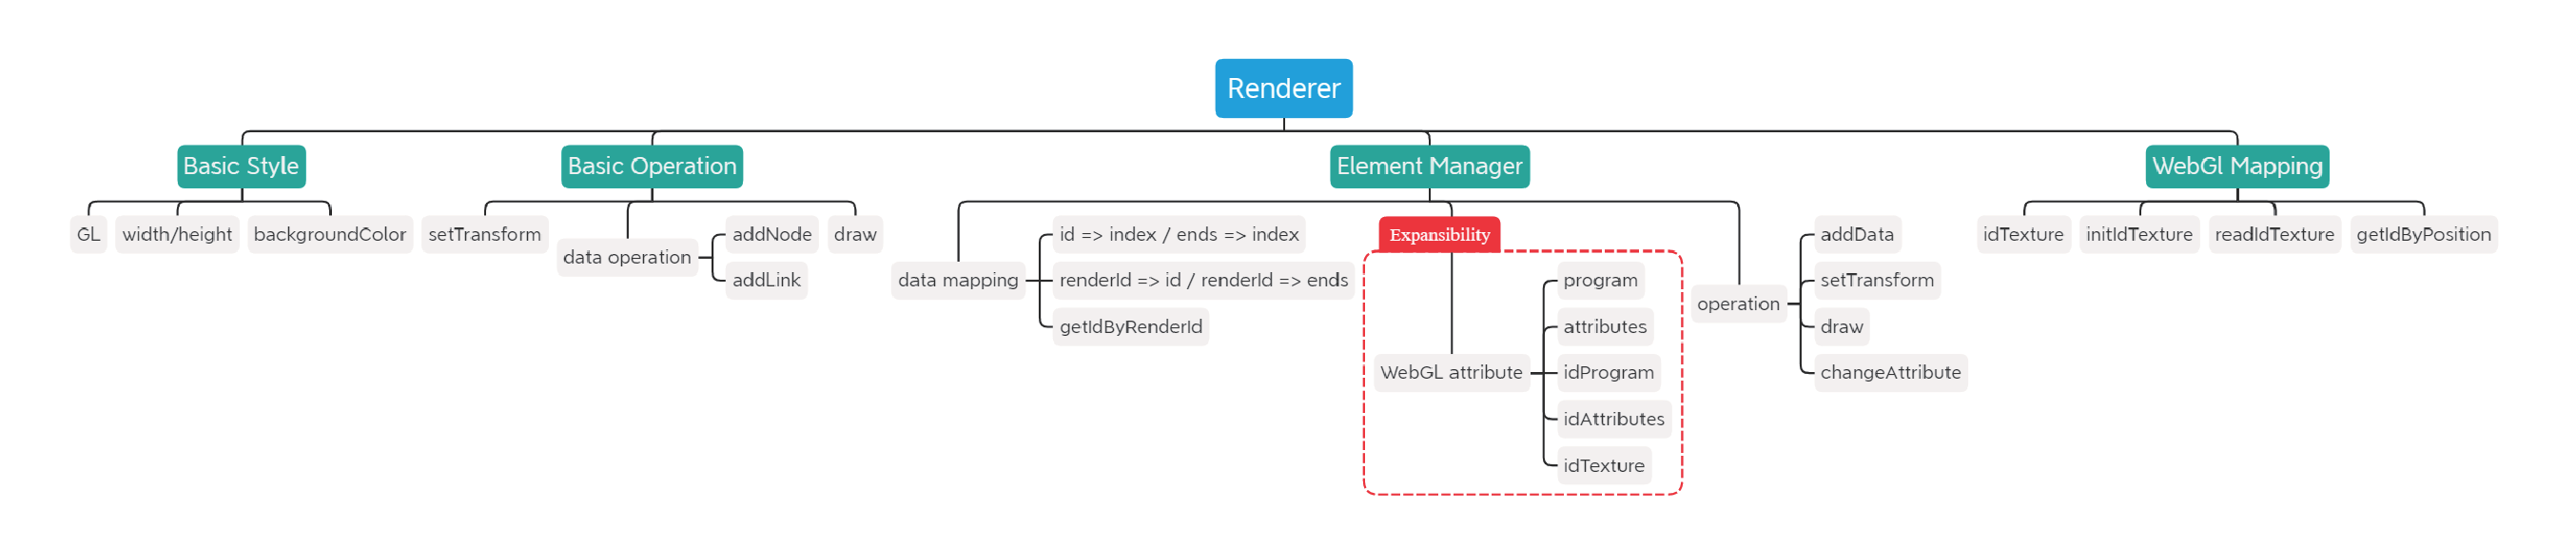
\includegraphics[width=\linewidth]{fig/xmind-01.eps}
    \caption{
        \name designs: \name consists of three parts: core engine, plugins, and library interface.
    }
    \label{fig:design}
\end{figure*}

\begin{figure}[htbp]
    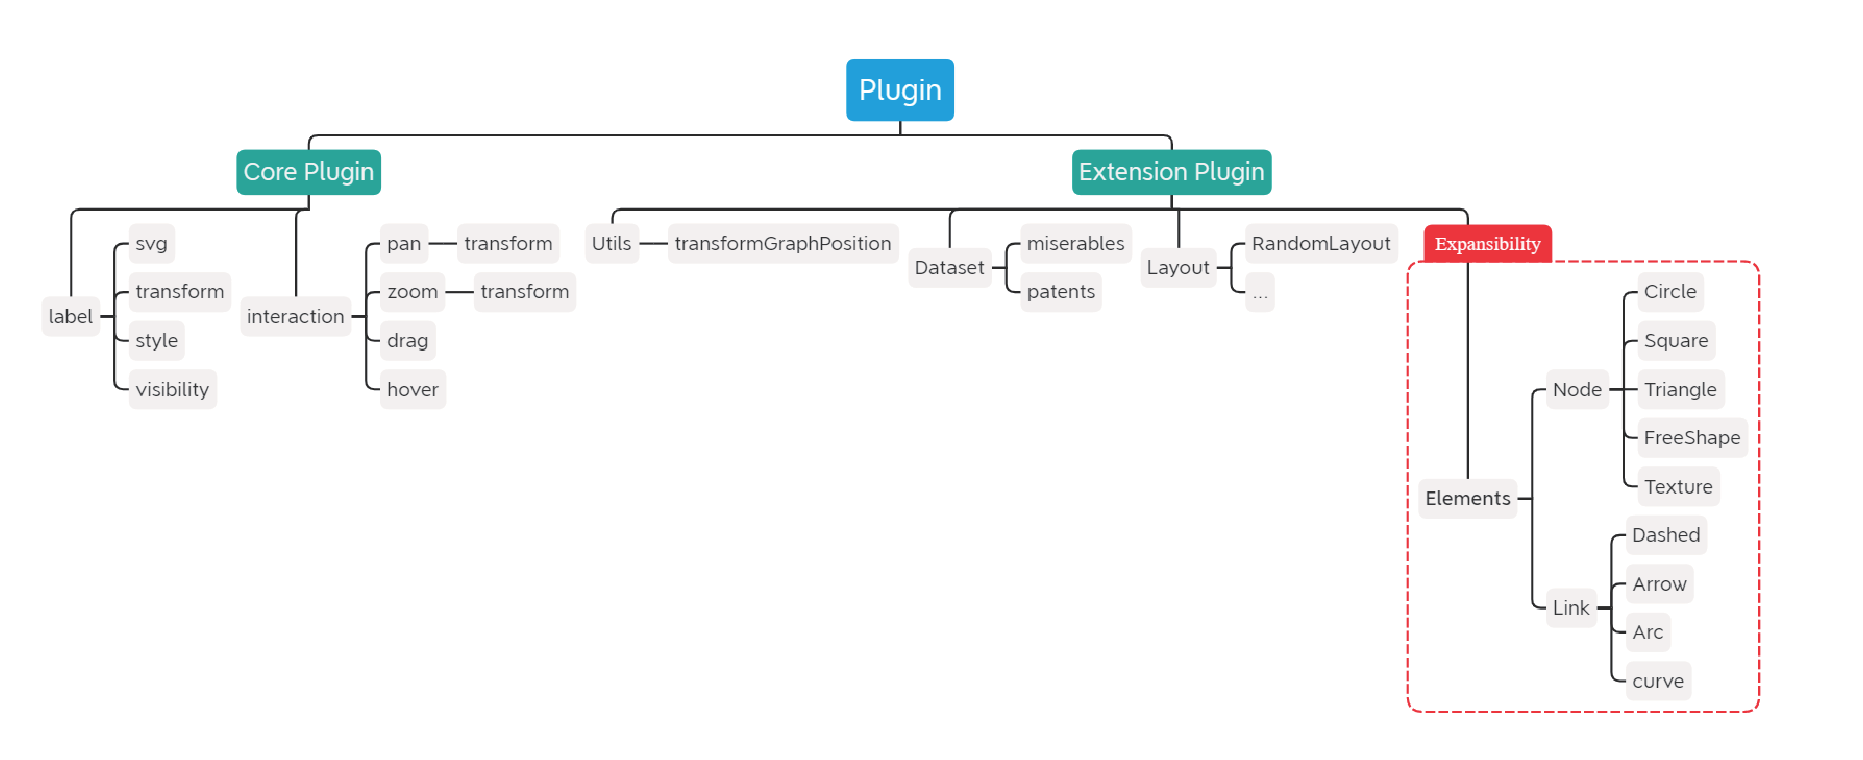
\includegraphics[width=\linewidth]{fig/xmind-02.eps}
    \caption{
        \name designs: \name consists of three parts: core engine, plugins, and library interface.
    }
    \label{fig:design}
\end{figure}
\begin{figure}[htbp]
    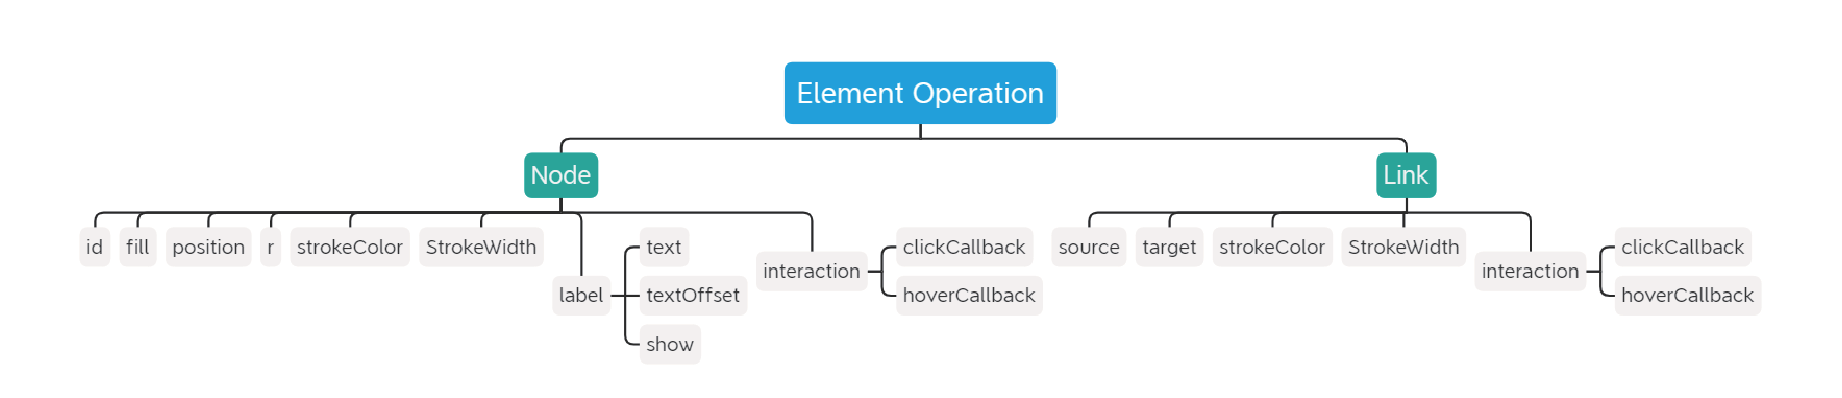
\includegraphics[width=\linewidth]{fig/xmind-03.eps}
    \caption{
        \name designs: \name consists of three parts: core engine, plugins, and library interface.
    }
    \label{fig:design}
\end{figure}
\begin{figure}[htbp]
    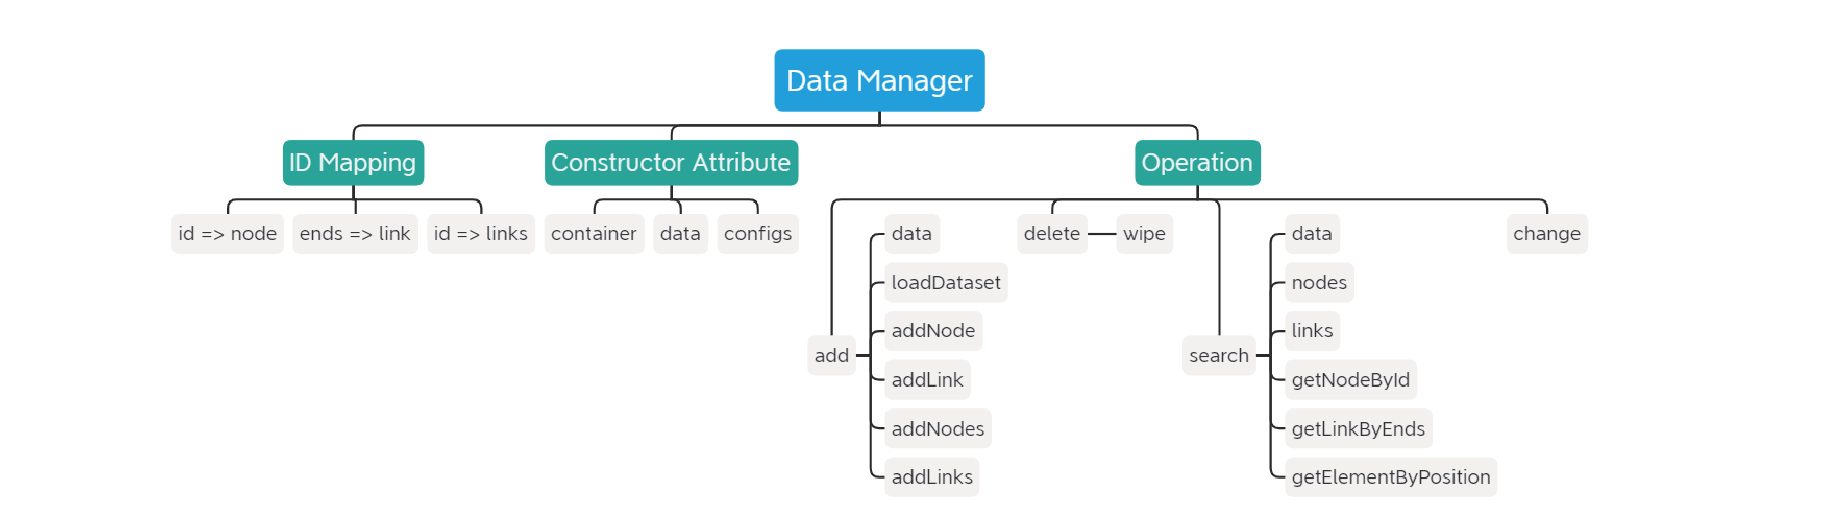
\includegraphics[width=\linewidth]{fig/xmind-04.eps}
    \caption{
        \name designs: \name consists of three parts: core engine, plugins, and library interface.
    }
    \label{fig:design}
\end{figure}

\subsection {Design Requirements of \name}

\deleted[id=pan]{为了探索\name的设计空间,我们采访了3个图可视化相关的专家,调研了一系列图可视化的工具,包括 Gephi, Cytoscape.js, Sigma.js, GraphViZ,总结了如下高性能节点链接图可视化的设计需求:}

\added[id=pan] {To explore the design space of \name, we interviewed 3 graph visualization experts, investigated 6 graph visualization tools including Gephi~\cite{DBLP:conf/icwsm/BastianHJ09}, Pajek~\cite{DBLP:reference/snam/BatageljM14}, SNAP~\cite{leskovec2016snap}, Sigma.js~\cite{DBLP:journals/jossw/Coene18}, GraphViZ~\cite{Ellson03graphvizand}, and Cytoscape.js~\cite{DBLP:journals/bioinformatics/FranzLHDSB16}. We summarized the following design requirements for high-performance node-link diagram visualization: }

\begin{itemize}
\item \deleted[id=pan]{\textbf{需要对拥有大量可视化元素的节点链接图提供高刷新率}: 根据我们对三位图可视化专家的采访,他们认为【对超过10万元素的大规模图有30fps以上的渲染速度】才能认为其对大规模节点链接图提供了高性能渲染的能力。}
\item \deleted[id=pan]{\textbf{需要有抽象的图模型来帮助控制图可视化}: 为了简化开发者对于可视化的操作,\name需要一个抽象图模型来控制图可视化而非直接控制图可视化的元素。该模型需要支持图的以下几点特性:}
\begin{itemize}
    \item \deleted[id=pan]{\textbf{链接关联节点}: }
    \item \deleted[id=pan]{\textbf{邻节点和邻接边的可访问性}: }
    \item \deleted[id=pan]{\textbf{基本图度量的计算}: }
    \item \deleted[id=pan]{\textbf{基本图论算法的支持}: }
\end{itemize}
\item \deleted[id=pan]{\textbf{支持不同节点和链接的样式}:}
\item \deleted[id=pan]{\textbf{需要提供多种布局功能和自定义布局插件}:}
\item \deleted[id=pan]{\textbf{需要提供基本的文本标签渲染和自定义标签}:}
\item \deleted[id=pan]{\textbf{需要提供基础交互模型}:}
\end{itemize}


\name aims to help users rapidly and efficiently construct network visualization applications.
Specifically, \name consists of three parts: the core engine, plugins, and library interface (\autoref{fig:design}).
The core engine contains the data manager for maintaining nodes and links and the renderer for leveraging GPU processing power to render a large-scale network.
The plugins are employed to increase and expand more requirements and functions.
The library interface aims to help developers rapidly construct applications with friendly and concise APIs.


\subsection{Core Engine}
The core engine aims to render large-scale network based on WebGL and maintains the primary network information for rapidly editing operations.
It consists of the data manager and the renderer.

\subsubsection{Data Manager}
The data manager supports a series of interface corresponding network structure.
It is used to achieve nodes or links operations, including adding, deleting, searching, and editing.
Node-links and link-nodes mapping tables are also supported for accelerating search and locate.
At the same time, the data manager has a build-in network data set for developers to get started quickly.

\subsubsection{Renderer}
The renderer aims to render basic elements: nodes and links. It focuses on the efficiency of rendering massive data on the browser platform. As the highest performance graphics rendering API of browser platform, \name uses WebGL as the bottom rendering.
However, WebGL programming is still hard and complex.
The WebGL API is encapsulate
In order to reduce the program execution time as much as possible, the basic WebGL API is only encapsulated to meet the most basic data processing and rendering.
Specifically, the renderer uses three strategies to improve rendering efficiency.

\begin{itemize}
\item \textbf{Batch}: The renderer contains a batch drawing element instance. Considering that most of the elements of the network are the same, but the location information is different. The renderer creates an instance of an element and draws it in the batch process to reduce the consuming time of the rendering process.

\item \textbf{Shader}: The renderer uses Shader function to control the shape render. Each node's shape usually needs to be defined as a circle, square, ellipse, and so on. However, the complex shape will cause a serious effect on rendering performance.
\name exploits the powerful Shader function to define and render shape in GPU with batch processing.

\item \textbf{Modify as needed}: The renderer supports manual rendering function for developers.
The main attributes of elements, including positions, color, and texture, are stored into different buffers of GPU.
When attributes of elements need to be Modified, the renderer can refresh corresponding buffers rather getting attributes from the data manager. And then, developers can refresh the network by supported function. The time consuming of getting attributes from the data manager can be omitted.

\item \textbf{Element positioning}: The renderer has an elements positioning function for supporting elements search and interaction. For improving user interaction efficiency, the renderer uses the WebGL Texture to record the screen pixel position of each element.
The time consuming of elements positioning has great improvement compared with index search and spatial index tree.
The time complexity of the function is $O(1)$.

\end{itemize}

\subsection{Plugin module}
The goal of the plugin modular is to enhance future expansions.
For supporting more features and requirements, \name designs the plugin modular to employ new improvements or functions.
At the same time, it can isolate the core modular from the rest.
For now, the plugin module includes:
\begin{itemize}
    \item \textbf{Interaction: } It supports binding interaction events and callback functions of elements. Interaction events contain basis events of edges and nodes such as Hover, MouseDown, Click, etc.
    \item \textbf{Layout: } It contains build-int layouts and allows users to use custom layouts.

\end{itemize}

\subsection{Library Interface}
The library interface aims to support concise and efficient API for users to build large-scale network visual analysis applications quickly.
Users do not need to touch the underlying WebGL rendering programming. Humanized and simple API can be called to config data and render network.
Specifically, it includes three parts:
\begin{itemize}
    \item \textbf{Global: }It is used to define custom configs, such as the mount node, the default style of the canvas, and the default style of elements.
    \item  \textbf{Element: }It includes the data adding of nodes of edges and the attributes changing of elements.
    \item  \textbf{Plugin: }It aims to set up different plugins, such as layouts and interactions.
\end{itemize}

\section{Examples}
In this section, we show diverse examples to illustrate the usage of \name.
\begin{figure*}
    \includegraphics[width=\linewidth]{fig/ex5.eps}
    \caption{
        Illustrations of (a) the customized style, (b) the label plugin, (c) the lasso selection, (d) and (e) are two large-scale datasets.
%with 74,752 nodes 261,120 edges, and 35,590 nodes 572,915 edges
    }
    \label{fig:ex5}
\end{figure*}

\subsection{Basic Graph Drawing}
\autoref{fig:ex2} shows a basic case with three parts: initialization, loading data, and rendering. The \codeword{testData} illustrates the graph data format. In this example, the initialization part hangs the canvas to the document \replaced[id=kg]{``main''}{`main'}.
\begin{figure}
    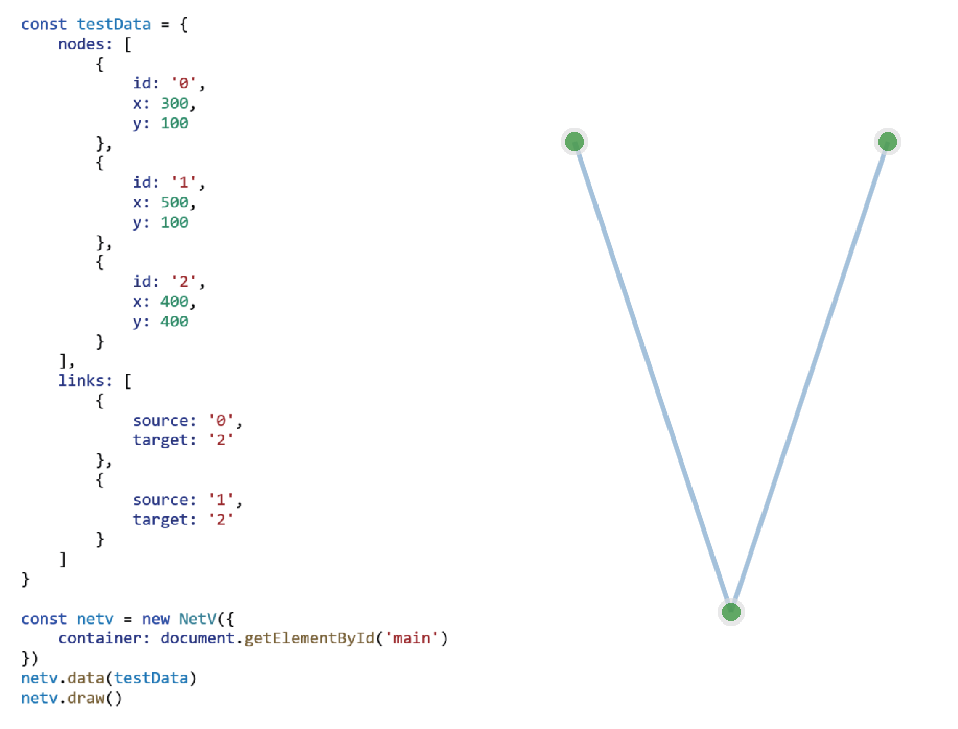
\includegraphics[width=\linewidth]{fig/ex2.eps}
    \caption{
        A basic unit of drawing three nodes and two edges.
    }
    \label{fig:ex2}
\end{figure}

\subsection{Customized Style}
The most important function of graph visualization is to draw a graph with different styles, \replaced[id=kg]{including}{such as} \added[id=kg]{the} color, stroke, radius, and position of elements.
\autoref{fig:ex5} shows the setting of customized styles by using \name. Developers can customize the style of each element and set the default style in the initialization part. In particular, \replaced[id=kg]{initialization}{initializzation} configuration items are set in the \replaced[id=kg]{``configs''}{`configs'}.


% \begin{figure}
%     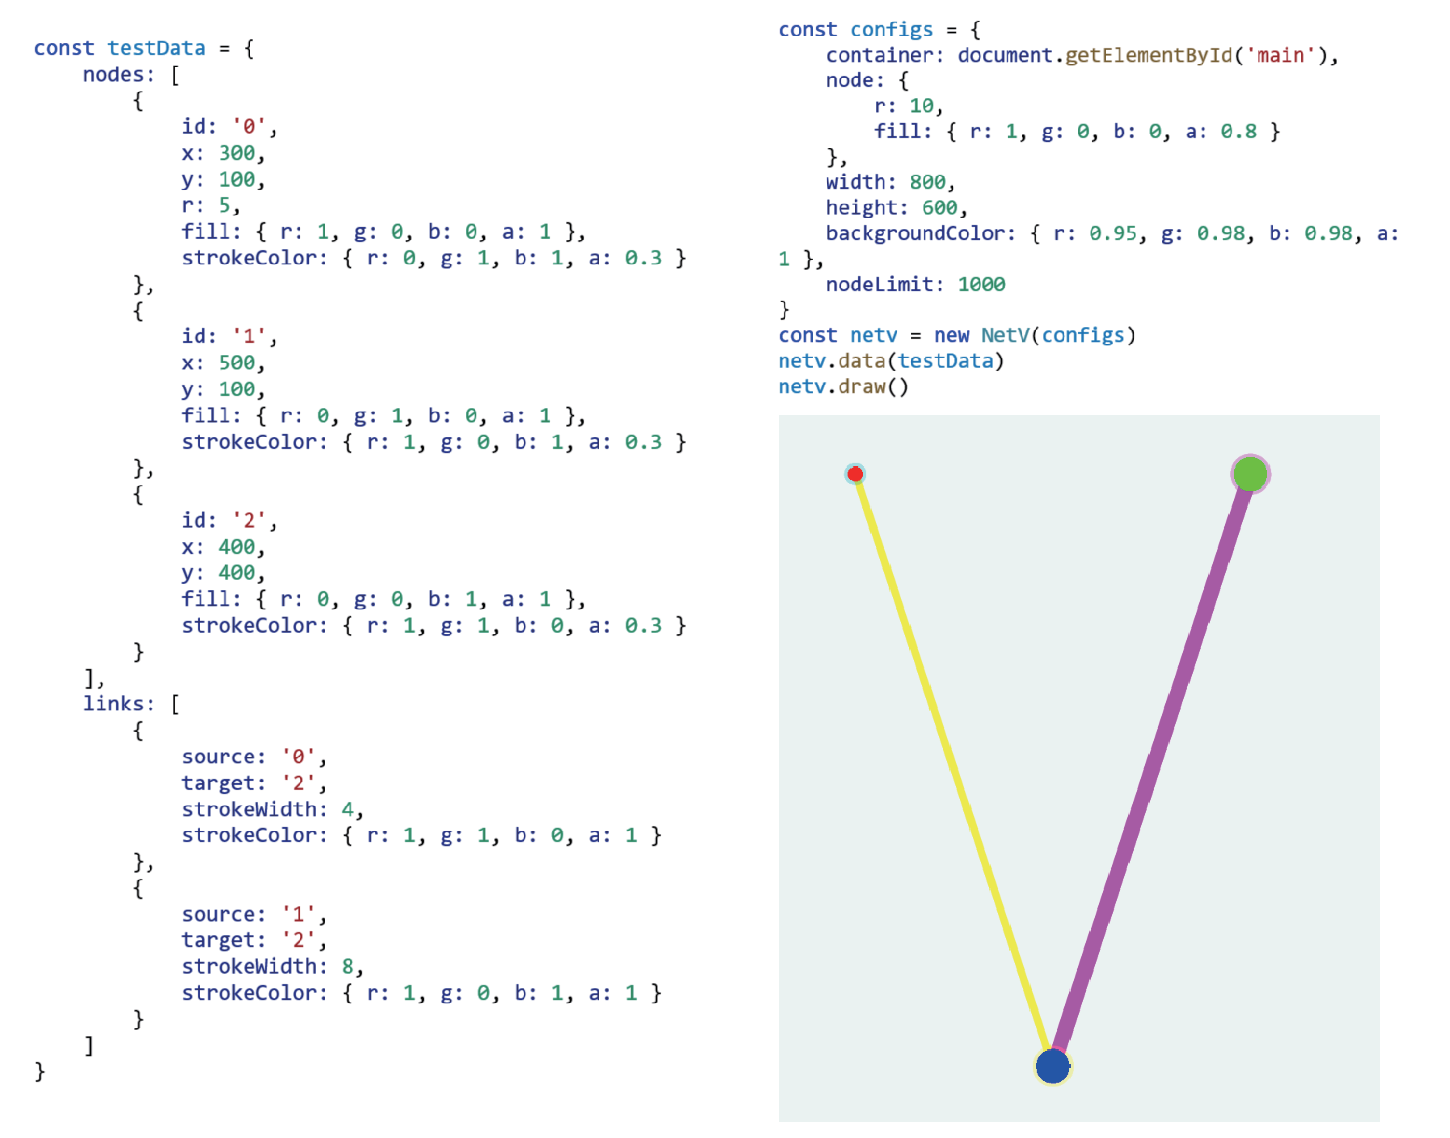
\includegraphics[width=\linewidth]{fig/ex1.eps}
%     \caption{
%         Customized style.
%     }
%     \label{fig:ex1}
% \end{figure}

% \subsection{Build-in datasets}
% \name supports build-in datasets for developers to construct a graph visualization (\autoref{fig:ex3}) quickly. The build-in datasets also support the attribute and the position of each node in the graph.
% developers can the radius and the color of nodes to encode different attributes of nodes.
% \begin{figure}
%     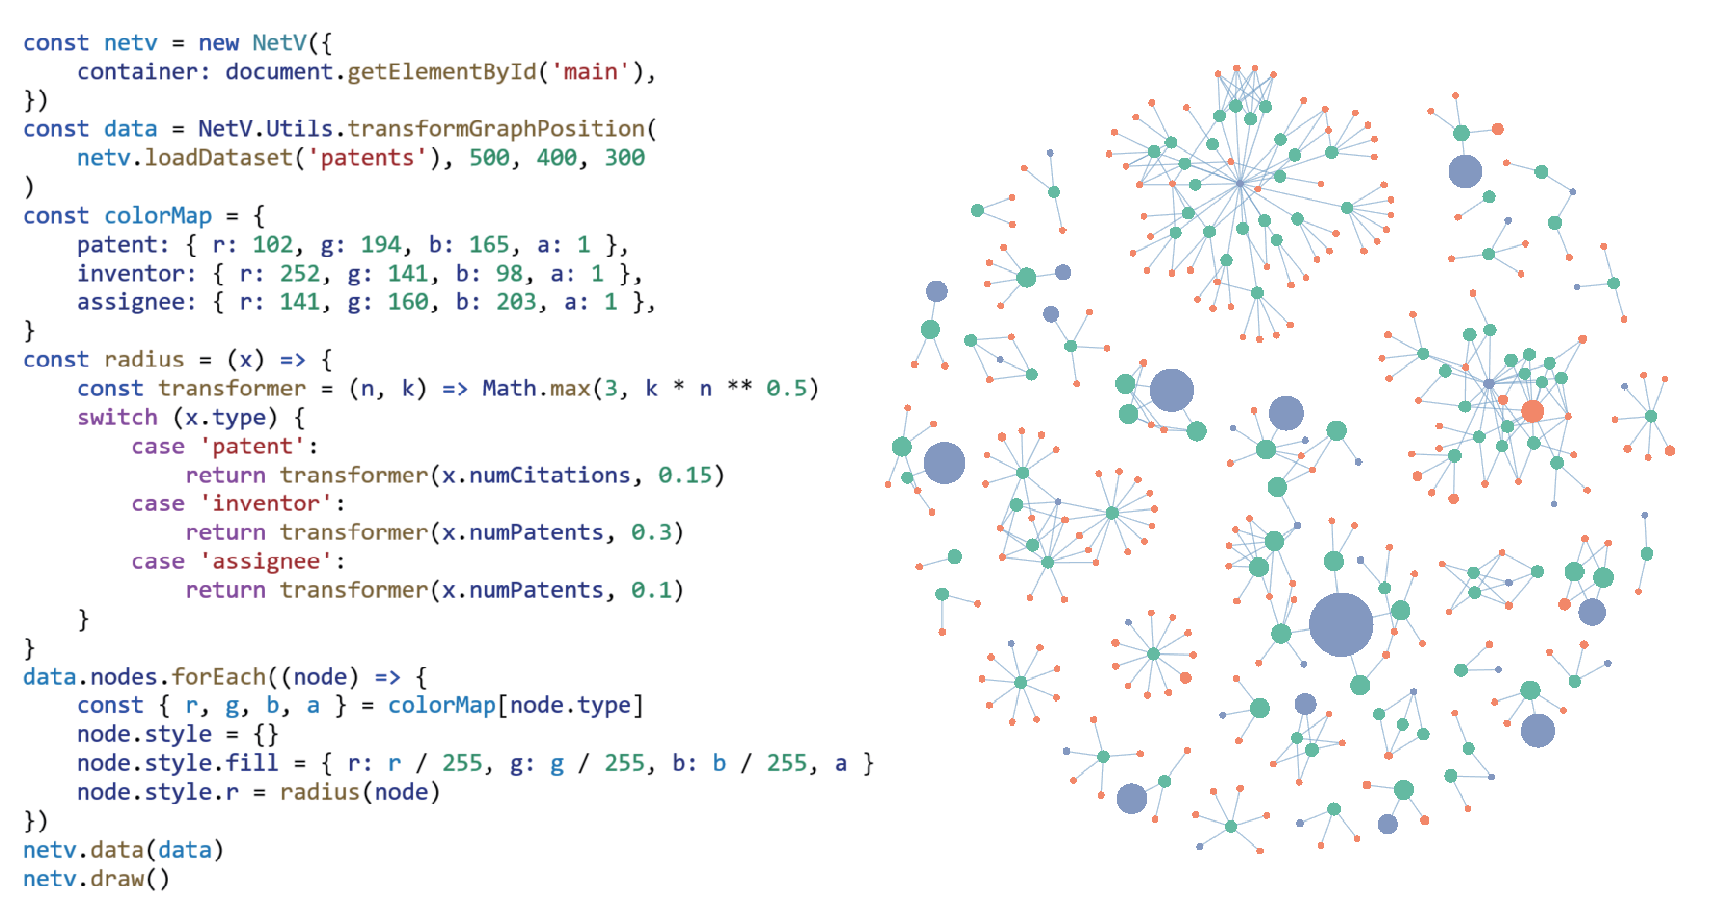
\includegraphics[width=\linewidth]{fig/ex3.eps}
%     \caption{
%         Build-in datasets.
%     }
%     \label{fig:ex3}
% \end{figure}

\subsection{Interaction}
A series of basic interactions are supported in \name, including pan, zoom, \added[id=kg]{and} \replaced[id=kg]{mouseover}{mousueover} \deleted[id=kg]{and so no}. \autoref{fig:ex8} (b) shows several \replaced[id=kg]{built-in}{build-in} interactions.

\subsection{Plugin}

\name supports showing labels (\autoref{fig:ex5} (b)) with different drawing techniques\added[id=kg]{,} such as SVG, Canvas, and WebGL. \name also supports lasso interaction (\autoref{fig:ex5} (c)) to select nodes and different layout algorithms. \autoref{fig:ex8} (a) shows \added[id=kg]{the} plugin configurations of the label, lasso, and layout.


\begin{figure}
    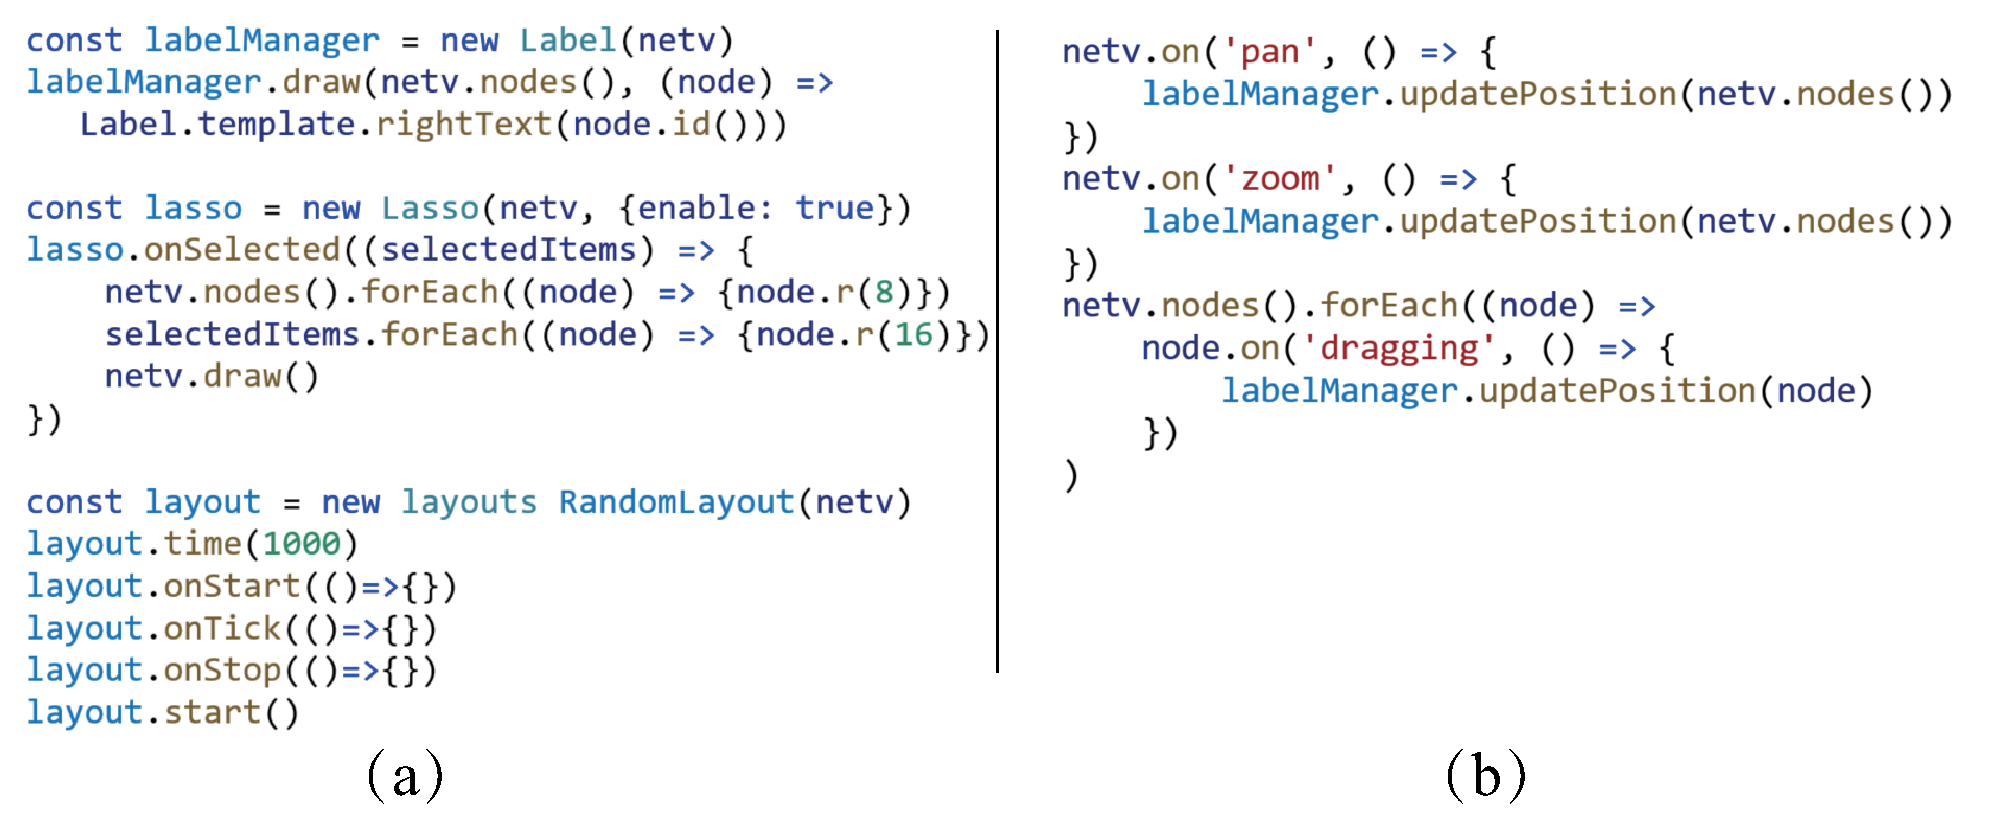
\includegraphics[width=\linewidth]{fig/ex8.eps}
    \caption{
        Code examples of (a) plugin configurations, and (b) build-in interactions.
    }
    \label{fig:ex8}
\end{figure}

% \subsection{Layout}
% \name supports various graph layout algorithms. Moreover, developers can implement by combining with external layouts such as D3.js (\autoref{fig:ex4} (a)), or by using \name plugins (\autoref{fig:ex4} (b)). When combining with external layouts, \name acts as a renderer to draw graph by layout results.
% When using \name layout plugins, it supports developers to controllers of all layout stages. \autoref{fig:ex5} (b) (c) (d) show the graph visualization with force-directed layout.
% \begin{figure}
%     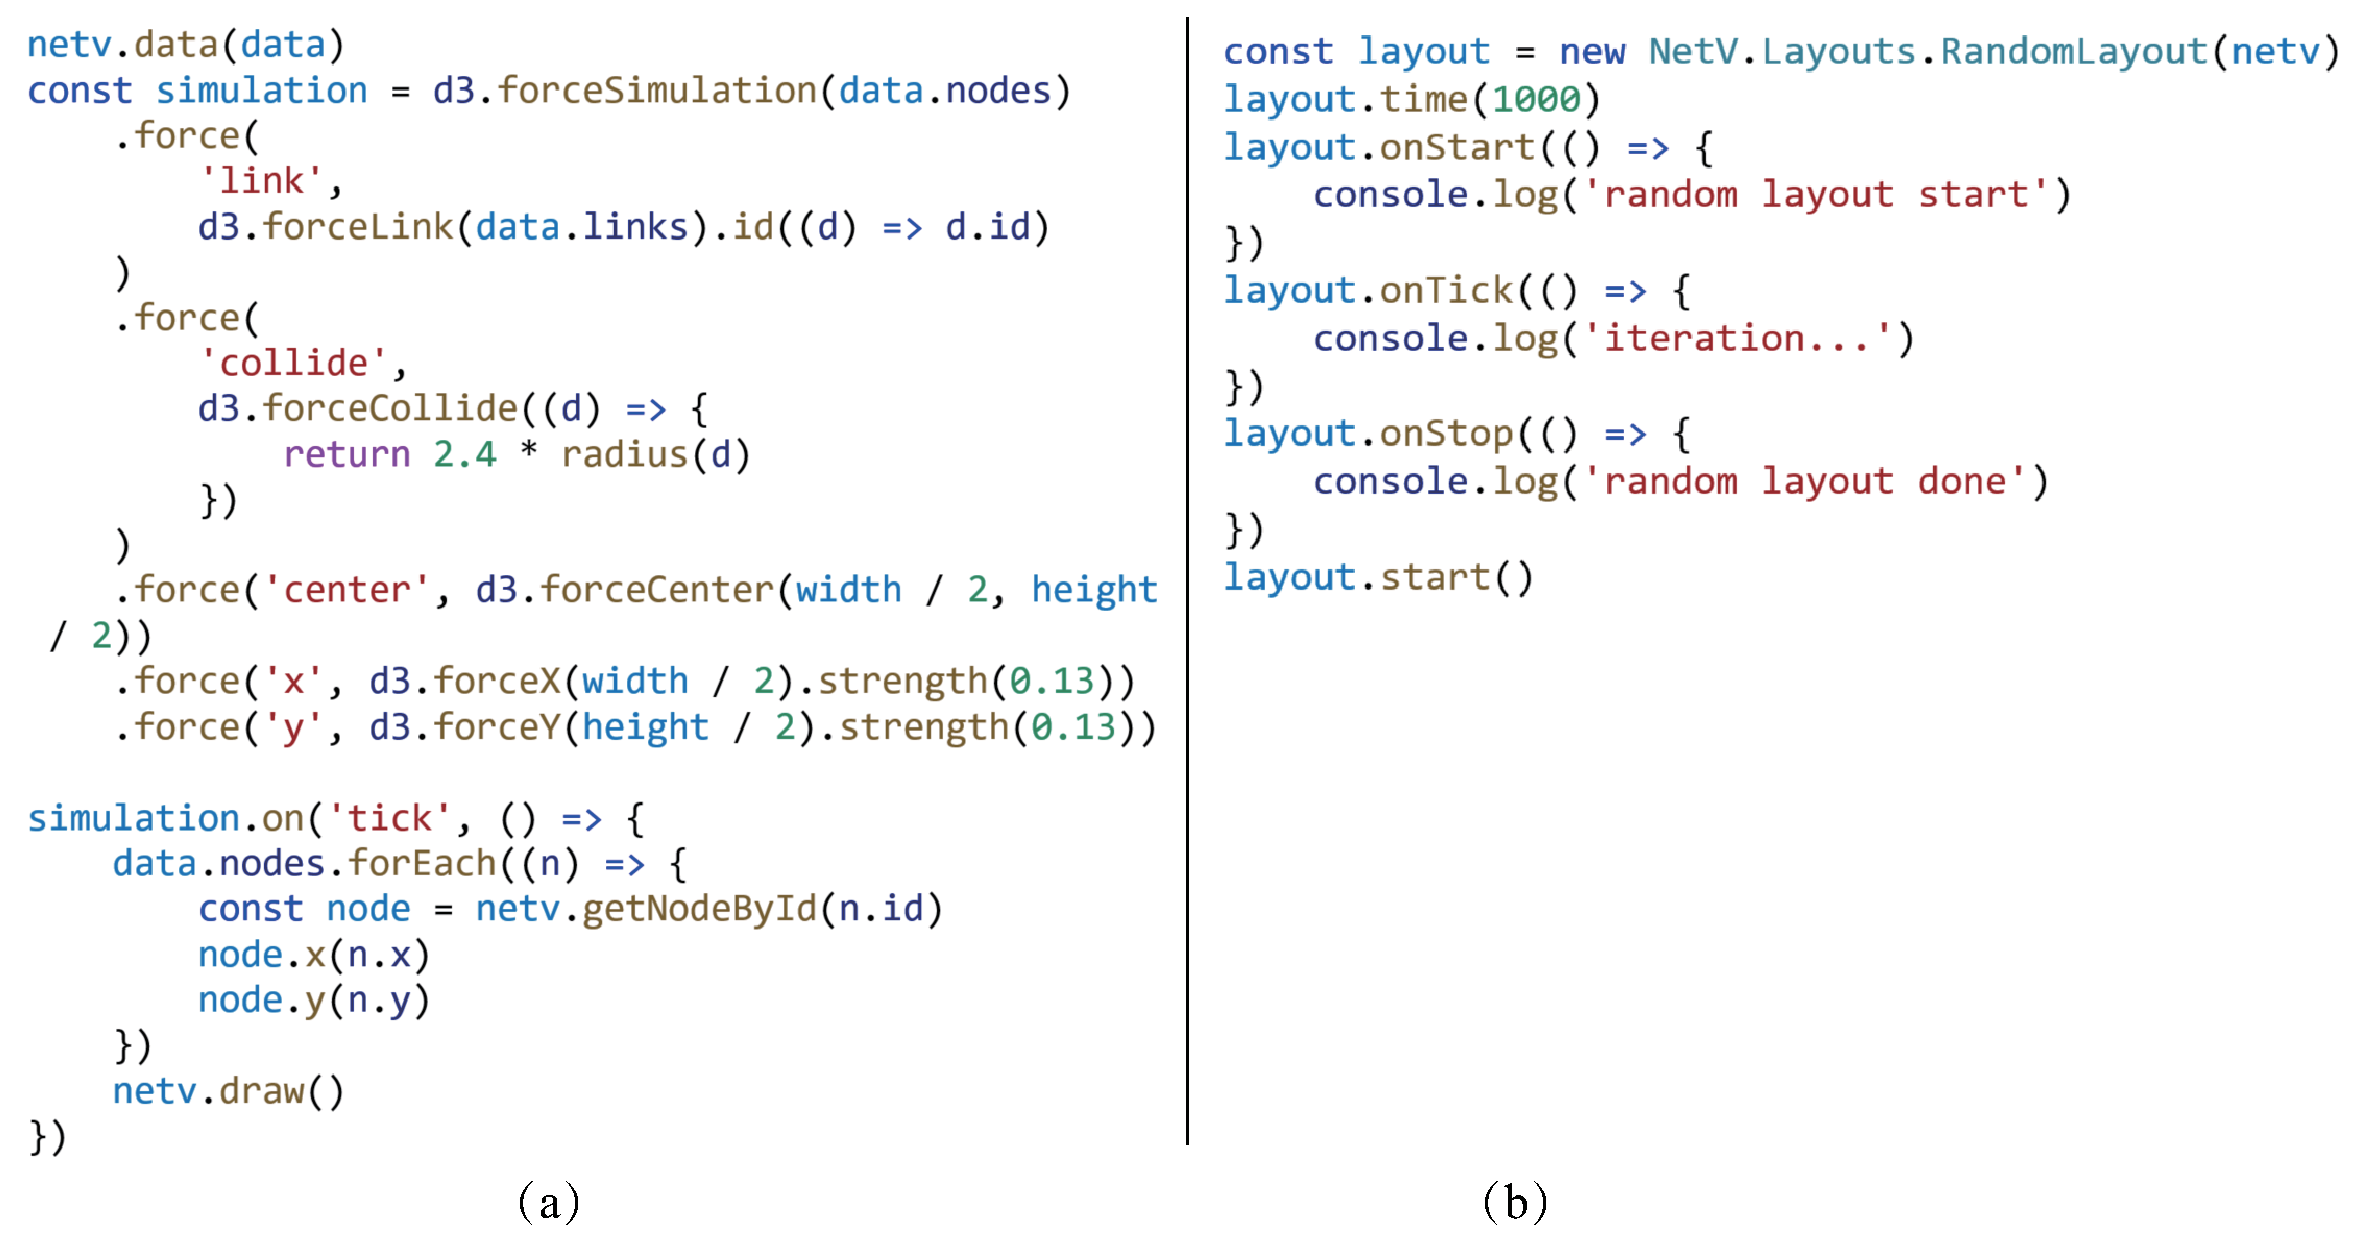
\includegraphics[width=\linewidth]{fig/ex4.eps}
%     \caption{
%         Layout. (a) Combining with D3.js. (b) Using \name plugins.
%     }
%     \label{fig:ex4}
% \end{figure}

\subsection{Large-\replaced[id=kg]{scale}{Scale} Graph}
\name aims to render large-scale graphs. \autoref{fig:ex5}(d) shows the graph visualization results of \replaced[id=kg]{the finan512}{Finan512} dataset~\cite{davis2011university} with 74,752 nodes and 261,129 edges. \autoref{fig:ex5}(e) shows the graph visualization results of \added[id=kg]{the} bcsstk31 dataset~\cite{davis2011university} with 35,590 nodes and 572,915 edges\replaced[id=kg]{.}{,} \deleted[id=kg]{Thanks to WebGL, }NetV.js can easily support \added[id=kg]{in} rendering millions of elements \added[id=kg]{due to its use of WebGL }.




% \begin{figure}
%     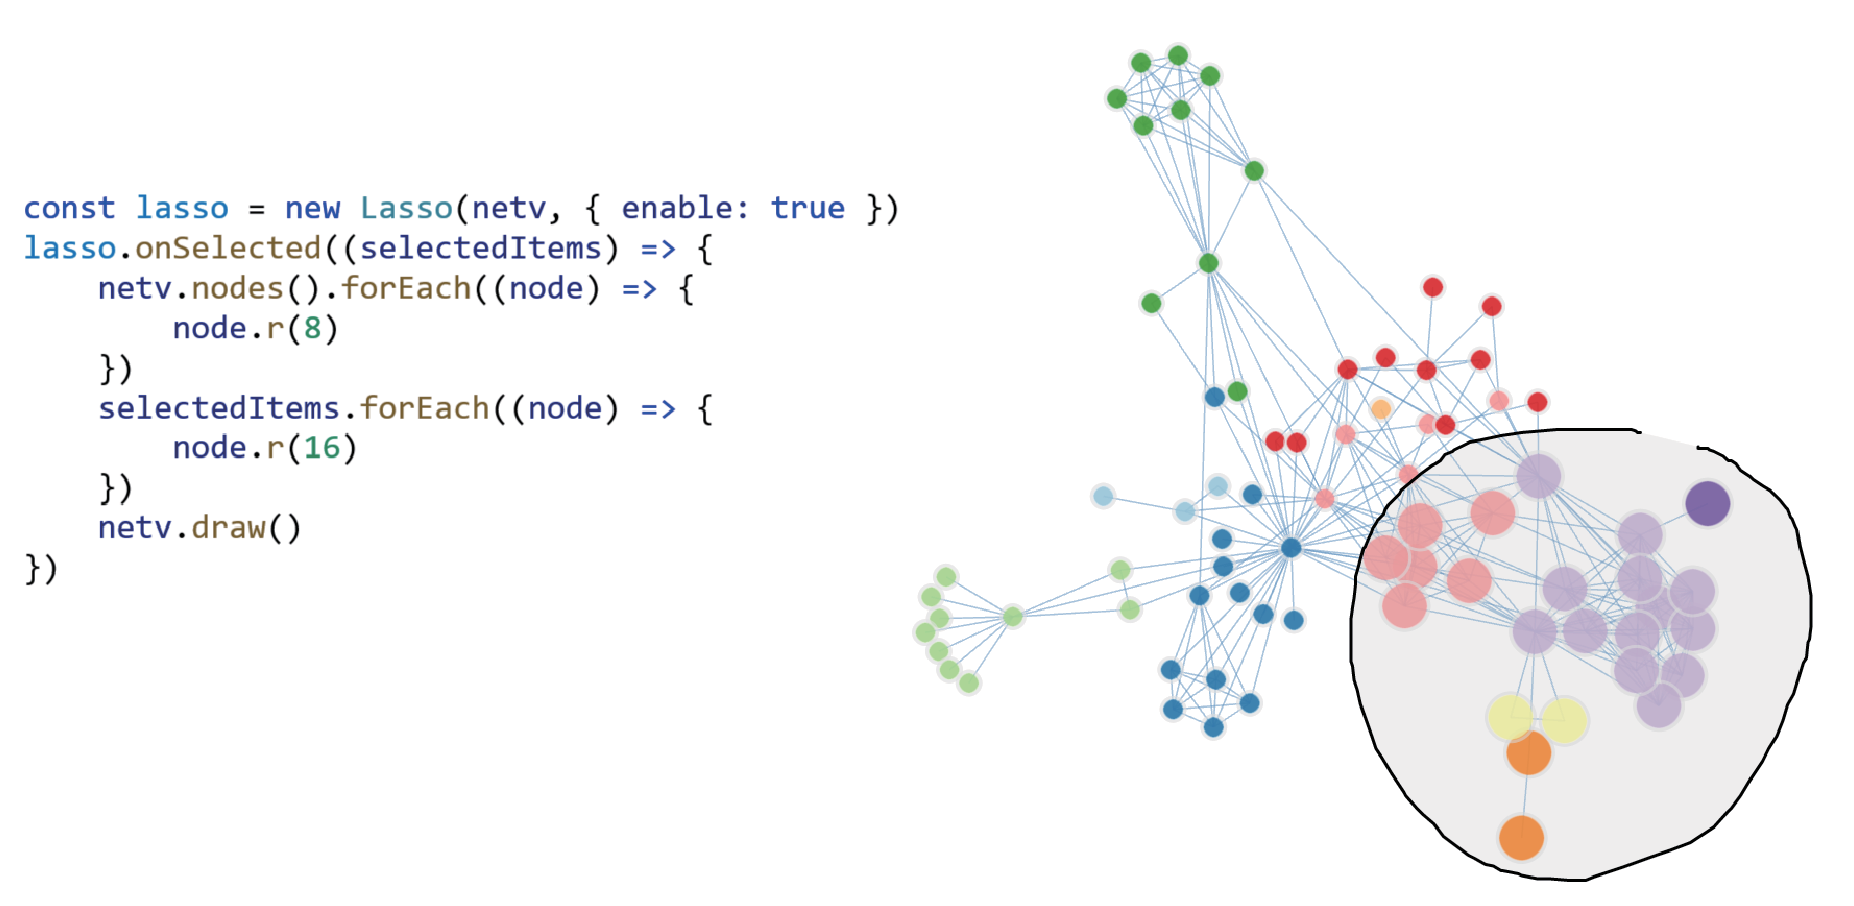
\includegraphics[width=\linewidth]{fig/ex7.eps}
%     \caption{
%         Label.
%     }
%     \label{fig:ex7}
% \end{figure}
\section{Experiment}\label{sec:experiment}
\autoref{fig:eva} shows the frame per second (FPS) over datasets with varied sizes of \name and other 5 tools\footnote{https://github.com/ZJUVAG/NetV.js/tree/benchmarks/benchmarks}, namely,  % We recorded the frame per second (FPS) experiment\footnote{https://github.com/ZJUVAG/NetV.js/tree/benchmarks/benchmarks} to test the rendering performance of \name with other popular tools and libraries which are supports graph rendering, including 
D3-SVG, D3-Canvas, Cytoscape.js, Sigma.js, and Stardust.js. In particular, \name, Sigma.js, and Stardust.js use WebGL. To simulate real-world graph data, we set the graph density as 20, which means the ratio of the number of edges to the number of nodes is 1 to 20. 
% The display refresh rate is 144Hz; the GPU is GTX 1060 with 6G.
Experiments are performed on a PC equipped with a GPU (NIVIDIA GTX 1060, 6G) and a monitor with a refreshing rate of 144 HZ.

Stardust.js, and D3-Canvas can render up to 100 thousand elements. \name can render more than 1 million elements with FPS greater than 1.

\begin{figure}[htbp]
    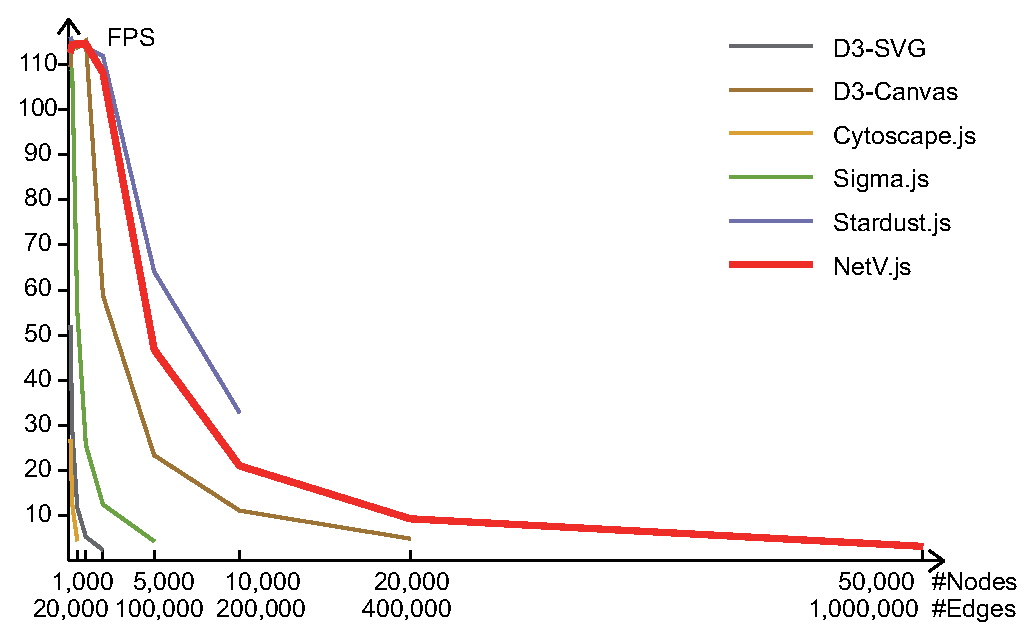
\includegraphics[width=\linewidth]{fig/eva.eps}
    \caption{
        Performance comparison among 6 toolkits.
    }
    \label{fig:eva}
\end{figure}

\section{Conclusion}
This paper presents NetV.js, an open-sourced, JavaScript-based, WebGL-based library that supports the rapid large-scale network rendering, interaction, and visualization. In the future, we plan to extend \name to support heterogeneous networks. We also plan to explore more visualization components and visual analysis algorithms for analyzing network data.

% \section{The Elsevier article class}

% \paragraph{Installation} If the document class \emph{elsarticle} is not available on your computer, you can download and install the system package \emph{texlive-publishers} (Linux) or install the \LaTeX\ package \emph{elsarticle} using the package manager of your \TeX\ installation, which is typically \TeX\ Live or Mik\TeX.

% \paragraph{Usage} Once the package is properly installed, you can use the document class \emph{elsarticle} to create a manuscript. Please make sure that your manuscript follows the guidelines in the Guide for Authors of the relevant journal. It is not necessary to typeset your manuscript in exactly the same way as an article, unless you are submitting to a camera-ready copy (CRC) journal.

% \paragraph{Functionality} The Elsevier article class is based on the standard article class and supports almost all of the functionality of that class. In addition, it features commands and options to format the
% \begin{itemize}
% \item document style
% \item baselineskip
% \item front matter
% \item keywords and MSC codes
% \item theorems, definitions and proofs
% \item lables of enumerations
% \item citation style and labeling.
% \end{itemize}

% \section{Front matter}

% The author names and affiliations could be formatted in two ways:
% \begin{enumerate}[(1)]
% \item Group the authors per affiliation.
% \item Use footnotes to indicate the affiliations.
% \end{enumerate}
% See the front matter of this document for examples. You are recommended to conform your choice to the journal you are submitting to.

% \section{Bibliography styles}

% There are various bibliography styles available. You can select the style of your choice in the preamble of this document. These styles are Elsevier styles based on standard styles like Harvard and Vancouver. Please use Bib\TeX\ to generate your bibliography and include DOIs whenever available.

% Here are two sample references: \cite{Feynman1963118,Dirac1953888}.

\section*{References}

\bibliography{mybibfile}
\end{CJK}
\end{document}